%%============
%%  ** Author: Qirong ZHANG
%%  ** Date: 2021-12-21 21:54:40
%%  ** Github: https://github.com/ShepherdQR
%%  ** LastEditors: Qirong ZHANG
%%  ** LastEditTime: 2024-12-02 23:15:36
%%  ** Copyright (c) 2019 Qirong ZHANG. All rights reserved.
%%  ** SPDX-License-Identifier: LGPL-3.0-or-later.
%%============






\documentclass[UTF8]{../06-Physics}
\begin{document}

\title{06-03-Mechanics}
\date{Created on 20220605.\\   Last modified on \today.}
\maketitle
\tableofcontents


\chapter{Introduction}

% \subsection{牛顿力学}
% \subsection{固体力学}
% \subsection{空气动力学}
% \subsection{流体动力学}

\chapter{Classic Mechanics}

\section{Classical Mechanics}


\subsection{Center of Mass}

Algebra defination $\boldsymbol r_c := \frac{\sum m_i \boldsymbol r_i}{\sum m_i} $, it relays to the choice of the coordinate system. If the map of the two coordinate systems is $T: S \rightarrow S'$, the matrix is orthogonal matrix, and $m_i$ has no inflence to the space, $\boldsymbol r'_c = T\boldsymbol r_c$.

The operator $\boldsymbol r_c $ simplifies the calculation, $(\sum m_i)\boldsymbol r_c = \sum m_i \boldsymbol r_i$.
We define the energy of the system like this, the whole energy $E_{all} := \sum \frac{1}{2} m_i \boldsymbol {v}_i^2$, the explicit energy $E_{ext} = \frac{1}{2} (\sum  m_i) \boldsymbol {v}_c^2$, the intrenal energy $E_{int} := \sum \frac{1}{2} m_i (\boldsymbol {v}_i- \boldsymbol {v}_c)^2$, because $\sum m_i \boldsymbol{v}_c^2-2\sum m_i \boldsymbol {v}_i \boldsymbol{v}_c = -\boldsymbol{v}_c^2 \sum m_i$, we have $E_{int} = E_{all} - E_{ext}$.

\subsection{Momentum}

$\sum m_i \boldsymbol {\ddot{r}}_i= \sum ({\boldsymbol F}_i + \sum \delta_{ij}\boldsymbol{f}_{i \leftarrow j})  = \sum \boldsymbol F_i $. We define momentum $\sum \boldsymbol{P}_i  =  \sum m_i \boldsymbol {\dot{r}}_i$, therefore, $\frac{d}{dt} \sum \boldsymbol{P}_i  = \sum {\boldsymbol F}_i$. [So the speed of light is always a const number, means that no other force can be applied to light?]

$\int \frac{d \boldsymbol{p}}{dt} = \boldsymbol{F}$, so $\int \boldsymbol{dp} = \int \boldsymbol F dt$.

\subsection{Rigid Body}
A rigid body changes from one position and orientation to another, the general movement can be represented as $\boldsymbol{v} = \boldsymbol \omega  \times \boldsymbol{r} $. 



\begin{proposition}[One fixed rotation axis]

Proof that the transformation of a rigid body has one fixed rotation axis. 

As shown in the figure, supposed that point A and B are on a sphere, and are transformed to $A'$ and $B'$, and two perpendicular bisector lines meets at point N, the point N can be transformed to $N'$, because that $\bigtriangleup ABN \cong  \bigtriangleup A'B'N'$, and moving on the orientable surface the triangular cannot transfered from $\bigtriangleup ABC$ into $\bigtriangleup ACB$, we say $N = N'$, the line $ON$ is the axis that doesn't move during the transformation.
    
The basis of the coordinate system $\boldsymbol{Z}^T := [e_1,e_2,e_3]$, represented as one line and three columns. The transformation of the basis $\boldsymbol{Z}' = \boldsymbol Z \boldsymbol{\Gamma }$, $\boldsymbol Z \boldsymbol{\Gamma } \boldsymbol{r}' =\boldsymbol Z \boldsymbol r $, so $ \boldsymbol{r}' = \boldsymbol{\Gamma } ^{-1}\boldsymbol{r}$, $\boldsymbol{\Gamma } \boldsymbol{\Gamma } ^{-1} = \boldsymbol{I}$ is easy to say when we write left in detail and considering that the $\boldsymbol{\Gamma }$ is the unit orthogonal base. Then the $\boldsymbol{\Gamma } \in SO_3$.
\end{proposition}

\begin{figure*}[h]
    \centering
    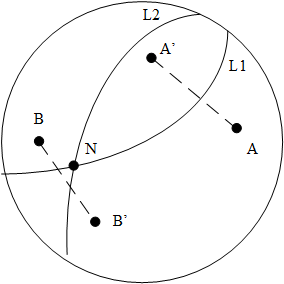
\includegraphics[width=0.5\textwidth]{../src/T0004_20211212_ProvehasOneAxis.png}
    \caption{[T0004:ProvehasOneAxis]}
    %%\label{fig:1}
\end{figure*}

The eigen value of $\boldsymbol{\Gamma }$, $\left\lvert \boldsymbol{\Gamma }-\boldsymbol{\lambda I}\right\rvert = \boldsymbol{0}$, so $-x^3 +\alpha x^2 +\beta x +1 = 0$, since the image of the function is continuous through $(-\infty , + \infty )$, it must have one root. 1 is one of the root. If the three roots are all real, they are all 1, or 1,-1,-1. If the rest two roots are virtual, they are $e^{i\theta},e^{-i\theta}$, so $T \phi = e^{i\theta} \phi $. 



\begin{equation}
    \begin{split}
    &\Gamma (\phi_1 + i \phi_2)   = e^{i\theta}(\phi_1 + i \phi_2) ,\\
    & \Gamma (\phi_1 - i \phi_2)   = e^{-i\theta}(\phi_1 - i \phi_2) \\
    &therefore:\\
    & \Gamma (\phi_1 ) = \cos(\theta) \phi_1  - \sin(\theta) \phi_2, \\
    &  \Gamma (\phi_2) = \sin(\theta) \phi_1  +\cos(\theta) \phi_2\\
\end{split}
\end{equation}
$\theta$ is the rotation angle.







\subsection{Anglar Momentum}
$\boldsymbol{L}_i := \boldsymbol{r}_i \times \boldsymbol{p}_i  $, with the defination of $\boldsymbol{p}$, we have $\sum \boldsymbol{L}_i  =\sum m_i \boldsymbol{r}_i \times \boldsymbol{v}_i$, and $\sum \boldsymbol{L}_i  =\sum \boldsymbol{r}_i \times \boldsymbol{F}_i + \sum \boldsymbol{r}_i \times \sum_j \boldsymbol{f}_{i \leftarrow j}$. Since $\sum(\boldsymbol{r}_i -\boldsymbol{r}_j) \times \boldsymbol{f}_{i \leftarrow j}  = 0$, we have $\sum \boldsymbol{L}_i  =\sum \boldsymbol{r}_i \times \boldsymbol{F}_i $. We also call that Torque.





\section{牛顿定律、达朗伯原理}
\section{力学中的数学方法}
\section{量纲分析与相似理论}



\section{Reference}

\subsection{Todo}
%%https://wuli.wiki/changed/HerMat.html





\subsection{Tmeplate}

\subsubsection{Tmeplate}

\begin{theorem}[均值不等式]

    设$A,B$是两个实数, 则$2AB\leq 2 A^2+B^2$.
    
\end{theorem}

\begin{proof}[均值不等式]

    设$A,B$是两个实数, 则$2AB\leq 2 A^2+B^2$.
    
\end{proof}

The free fall ball ends at $[1-\vert (\mu k)^{-1} \pmod 2 -1 \vert ]kH $

\begin{figure*}[h]
    \centering
    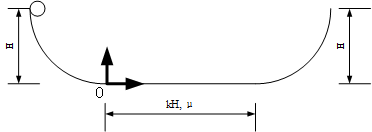
\includegraphics[width=0.5\textwidth]{../src/T0001.png}
    \caption{[T0001:]}
    \label{fig:1}
\end{figure*}




\chapter{理论力学 (一般力学 )}%% empty here




\chapter{振动理论}
    \subsection{线性振动}
    \subsection{非线性振动}
    \subsection{自激振动、参数振动}
    \subsection{随机振动}
    \subsection{有限自由度体系的振动}
    \subsection{弹性体的振动}
    \subsection{结构振动}
    \subsection{减振、隔振理论}
    \subsection{振动测量技术}


\chapter{连续介质力学 (变形体力学 )}
    \subsection{理性力学}





\chapter{固体力学}%% empty here



    
\chapter{流体力学}%% empty here



\chapter{流变学}
    \subsubsection{唯象理论}
    \subsubsection{统计理论}
    \subsubsection{非牛顿流体}
    \subsubsection{容积粘度}
    \subsubsection{正应力}
    \subsubsection{二次流}
    \subsubsection{应力松弛及反弹性应力松弛}


\chapter{爆炸力学}
\section{爆震 (爆轰 )理论}
\section{爆震波的传播}
    \subsection{在空中、水中及地下的传播}
    \subsection{在土及岩石中的传播}
    \subsection{在金属材料中的传播}
    \subsection{爆炸相似律理论和试验} 


\section{爆炸波与物体的相互作用}
    \subsection{爆炸波在空中、水中及地下的作用及防护}
    \subsection{爆炸波对各种建筑物的作用及防护}
    \subsection{爆炸波对各种机械及装备的作用及防护}

\section{爆炸波的观测技术}
\section{穿甲理论}
\section{应用爆炸力学}



\chapter{应用力学}







\chapter{Reference}

\end{document}

